\renewcommand*\chapterpagestyle{scrheadings}
\chapter{Introduction}

This project aims to deliver a versatile voice assistant implementation
compatible with various frontends. One such frontend,
developed concurrently with this project,
leverages the Qt framework\footnote{Qt Framework \cite{qt}}
to provide a user-friendly interface.

\section{Background and Motivation}
Voice assistants have seen steady growth in adoption,
yet they are often perceived as supplementary tools
rather than essential components of productivity.
This project addresses this limitation by developing a voice assistant solution
that enhances user workflows while maintaining minimal intrusiveness.
The implementation extends traditional voice assistant capabilities
with advanced features, including workspace management and seamless speech-to-text integration.

\section{Project Scope}
The project scope encompasses the following key objectives:
\begin{itemize}
    \item Achieving efficient processing with a target response latency of 1 second.
    \item Seamless integration into Linux window managers, enabling users to control their systems using voice commands.
    \item Support for both explicit recording and voice activation functionalities.
    \item Configurability, allowing users to select preferred algorithms, APIs, and output formats.
\end{itemize}

\section{System Architecture}
\subsection{Technology Considerations}
The choice of technology stack plays a critical role in achieving low response latency.
The initial prototype of the voice assistant was developed using Kotlin and Spring Boot\footnote{Spring Framework \cite{spring}},
which provided flexibility and ease of development.
However, as the project evolved and the stringent 1-second latency goal became a priority,
it became evident that a more performant approach was necessary.

To meet this performance requirement, the project transitioned to Rust.
Rust was chosen for its ability to produce highly optimized, natively compiled binaries,
making it ideal for low-latency applications.
Additionally, Rust's emphasis on memory safety and robust error handling
ensured the reliability of the application without sacrificing speed.
Prior experience with Rust further streamlined the development process,
solidifying its selection as the optimal choice for this project.

\subsection{Design}
The voice assistant system comprises two parallel projects:
the Rust backend (the focus of this thesis) and a Qt-based frontend
(developed concurrently but outside the scope of this thesis).
The frontend serves as the user interface layer,
providing efficient access to the backend's voice processing capabilities.

The backend is designed with a modular architecture to ensure flexibility and configurability.
Each stage of the processing pipeline is responsible for a specific aspect of the voice assistant's functionality,
enabling users to choose from a variety of processing methods—whether local, remote, paid, or free.

The backend consists of the following stages:

\begin{itemize}
    \item \textbf{Recording Stage:} Implements both local and remote recording capabilities:
    \begin{itemize}
        \item Local Recorder for direct hardware access.
        \item Remote Recorder for distributed setups.
    \end{itemize}
    \item \textbf{Transcription Stage:} Provides multiple transcription options:
    \begin{itemize}
        \item Local Whisper for offline processing.
        \item Cloudflare Whisper for edge computing.
        \item OpenAI Whisper for cloud-based processing.
    \end{itemize}
    \item \textbf{Processing Stage:} Implements various natural language processing (NLP) options:
    \begin{itemize}
        \item Local NLP for offline processing.
        \item Remote NLP for distributed processing.
        \item Cloudflare NLP for edge computing.
        \item OpenAI NLP for advanced language models.
        \item Regex Matcher for simple pattern matching.
    \end{itemize}
    \item \textbf{Output Stage:} Handles the final processing results and delivers them to the user.
\end{itemize}

This modular design ensures that the voice assistant can be tailored
to meet the specific needs and preferences of its users,
offering a robust and adaptable solution for voice interaction.

\begin{figure}[H]
    \centering
    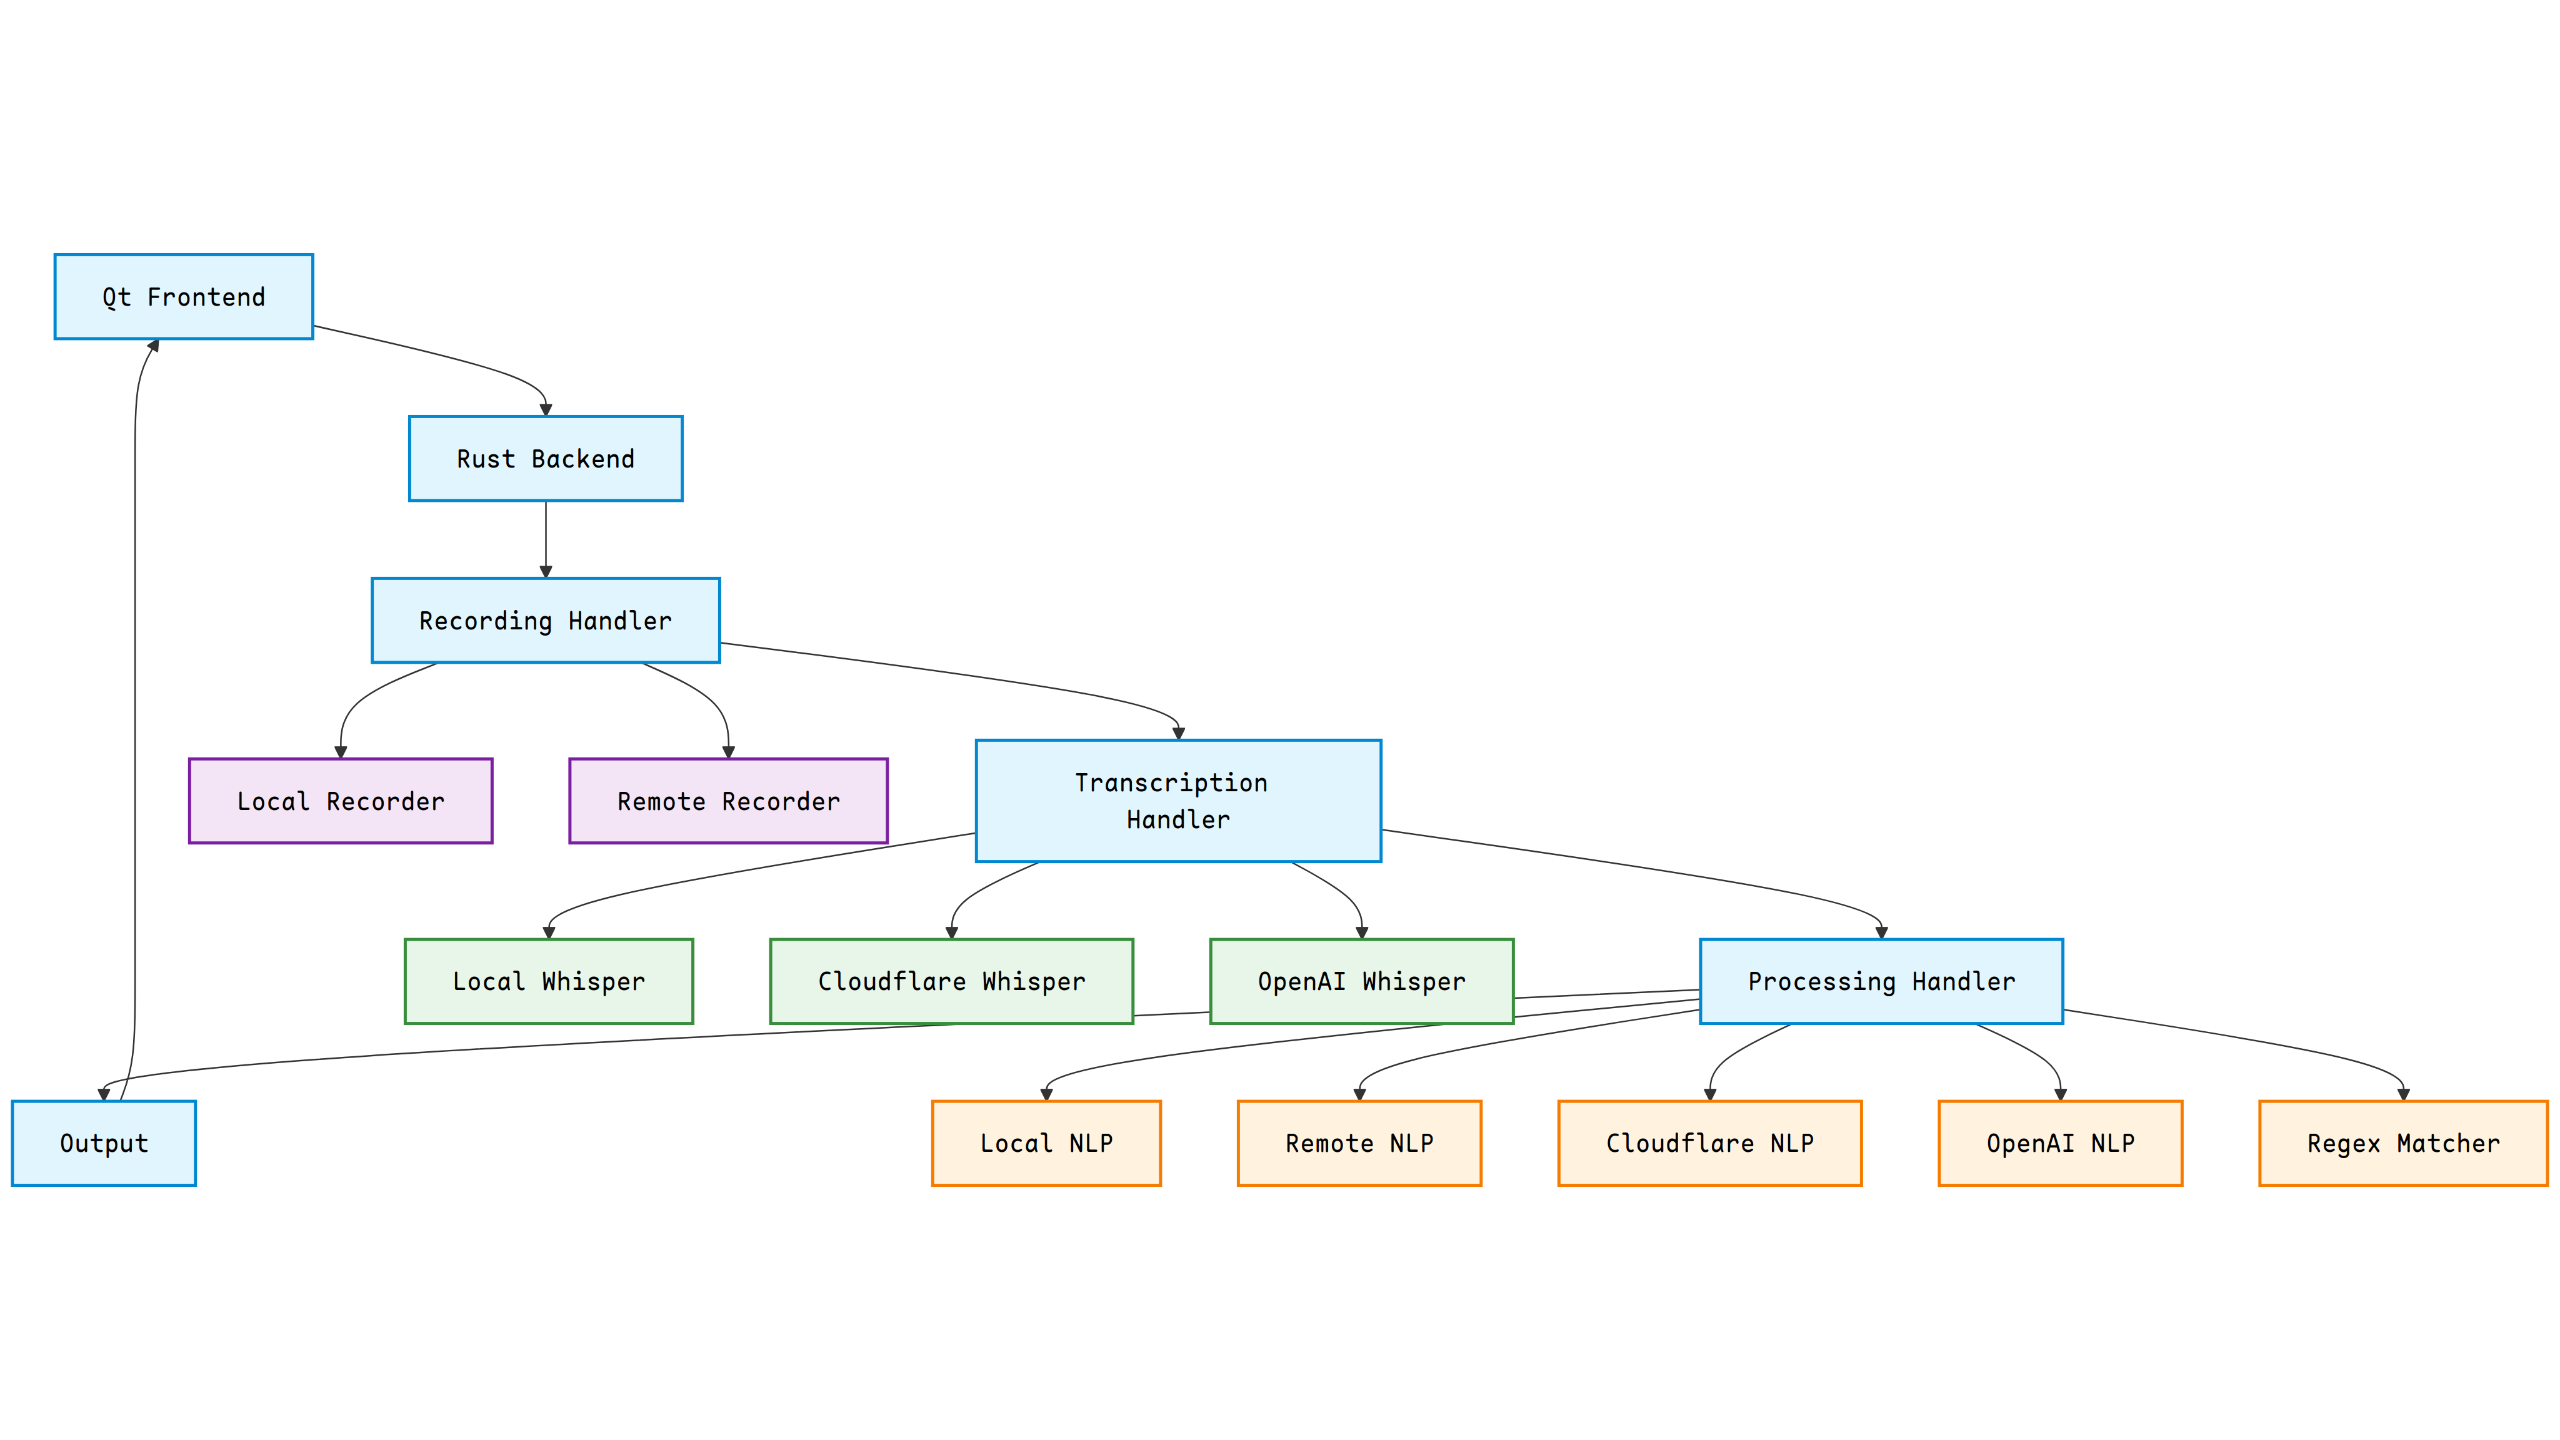
\includegraphics[width=\textwidth]{assets/stackchart}
    \caption{System architecture illustrating the Qt frontend (parallel project)
    and the Rust backend components (the focus of this thesis).
    The processing pipeline flows from the frontend through various backend stages,
    each offering multiple implementation options.}
    \label{fig:design}
\end{figure}

\section{Integration of Artificial Intelligence}
The voice assistant employs artificial intelligence (AI) to process user requests and generate responses.
This implementation provides pattern-matching systems as well as machine learning (ML) techniques,
particularly large language models (LLMs), to provide a choice between response speed and contextual understanding.

\subsection{Fallback Response Generation}
When encountering requests beyond its current capabilities (e.g., \textit{"Order a pizza"}),
the system uses LLMs to generate helpful responses rather than generic errors. For example, instead of replying \textit{``Command not recognized,"},
the assistant might respond: \textit{``I cannot order food yet, but I can show you local pizza restaurants."}
This approach maintains conversational flow while honestly acknowledging system limitations.

\subsection{Input Processing Architecture}
The system uses two methods to interpret user input:

\begin{enumerate}
    \item \textbf{Pattern Matching}: Direct commands like \textit{``Set timer for 10 minutes"} can be matched to predefined templates for immediate execution
    \item \textbf{Machine Learning}: Complex or ambiguous phrases (e.g., \textit{``Will it rain in that city with the musical history museum?"})
    will fail pattern matching and require using LLMs. These models infer meaning from context, even when wording is unconventional
\end{enumerate}

While pattern matching can handle a large number of common queries instantly, machine learning can resolve edge cases requiring contextual awareness.
